%\documentclass[mathserif]{beamer}
\documentclass[handout]{beamer}
%\usetheme{Goettingen}
\usetheme{Warsaw}
%\usetheme{Singapore}
%\usetheme{Frankfurt}
%\usetheme{Copenhagen}
%\usetheme{Szeged}
%\usetheme{Montpellier}
%\usetheme{CambridgeUS}
%\usecolortheme{}
%\setbeamercovered{transparent}
\usepackage[english, activeacute]{babel}
\usepackage[utf8]{inputenc}
\usepackage{amsmath, amssymb}
\usepackage{dsfont}
\usepackage{graphics}
\usepackage{cases}
\usepackage{graphicx}
\usepackage{pgf}
\usepackage{epsfig}
\usepackage{amssymb}
\usepackage{multirow}	
\usepackage{amstext}
\usepackage[ruled,vlined,lined]{algorithm2e}
\usepackage{amsmath}
\usepackage{epic}
\usepackage{epsfig}
\usepackage{fontenc}
\usepackage{framed,color}
\usepackage{palatino, url, multicol}
\usepackage{listings}
%\algsetup{indent=2em}
\newcommand{\factorial}{\ensuremath{\mbox{\sc Factorial}}}
\newcommand{\BIGOP}[1]{\mathop{\mathchoice%
{\raise-0.22em\hbox{\huge $#1$}}%
{\raise-0.05em\hbox{\L
\usepackage{fontenc}
\usepackage{framed,color}
\usepackage{palatino, url, multicol}
\usepackage{listings}
%\algsetup{indent=2em}
\newcommand{\factorial}{\ensuremath{\mbox{\sc Factorial}}}
\newcommand{\BIGOP}[1]{\mathop{\mathchoice%
{\raise-0.22em\hbox{\huge $#1$}}%
{\raise-0.05em\hbox{\Large $#1$}}{\hbox{\large $#1$}}{#1}}}
\newcommand{\bigtimes}{\BIGOP{\times}}
\vspace{-0.5cm}
\title{Introduction to Statistical Inference}
\vspace{-0.5cm}
\author[Felipe Bravo Márquez]{\footnotesize
%\author{\footnotesize  
 \textcolor[rgb]{0.00,0.00,1.00}{Felipe José Bravo Márquez}} 
\date{ \today }
arge $#1$}}{\hbox{\large $#1$}}{#1}}}
\newcommand{\bigtimes}{\BIGOP{\times}}
\vspace{-0.5cm}
\title{Linear Regression}
\vspace{-0.5cm}
\author[Felipe Bravo Márquez]{\footnotesize
%\author{\footnotesize  
 \textcolor[rgb]{0.00,0.00,1.00}{Felipe José Bravo Márquez}} 
\date{ \today }


\begin{document}
\begin{frame}
\titlepage


\end{frame}


%%%%%%%%%%%%%%%%%%%%%%%%%%%



\begin{frame}{Introducción}
\scriptsize{
\begin{itemize}

 \item Un modelo de regresión se usa para modelar la relación de una variable dependiente $\mathbf{y}$ numérica con $n$ variables independientes $\mathbf{x}_1, \mathbf{x}_2, \dots, \mathbf{x}_n$. 
 
 \item A grandes rasgos queremos conocer el valor esperado de $\mathbf{y}$ a partir los valores de $\mathbf{x}$:
 \begin{displaymath}
 \mathbb{E}(y|x_1,x_2,\dots,x_n)
 \end{displaymath}

 
 \item Usamos estos modelos cuando creemos que la variable de respuesta $\mathbf{y}$ puede ser modelada por otras variables independientes también conocidas como covariables o atributos.
 
 \item Para realizar este tipo de análisis necesitamos un dataset formado por $m$ observaciones que incluyan tanto a la variable de respuesta como a cada uno de los atributos.
 
 \item Nos referimos al proceso de \textbf{ajustar} una función de regresión al proceso en que a partir de los datos inferimos una función de hipótesis $h$ que nos permite predecir valores de $\mathbf{y}$ desconocidos usando los valores de los atributos.

 
\end{itemize}



} 
 
\end{frame}


\begin{frame}{Introducción (2)}
\scriptsize{
\begin{itemize}
 
 \item A este proceso de ajustar una función a partir de los datos se le llama en las áreas de minería de datos y aprendizaje de máquinas como \textbf{entrenamiento}.

 \item En esas disciplinas se dice que las funciones \textbf{aprenden} a partir de los datos.
 
 \item Como necesitamos observaciones donde el valor de $\mathbf{y}$ sea conocido para aprender la función,  se le llama a este tipo de técnicas como técnicas de \textbf{aprendizaje supervisado}.
 
 \item Cuando $\mathbf{y}$ es una variable categórica hablamos de un problema de \textbf{clasificación}.
 

 
\end{itemize}


\begin{figure}[h!]
	\centering
	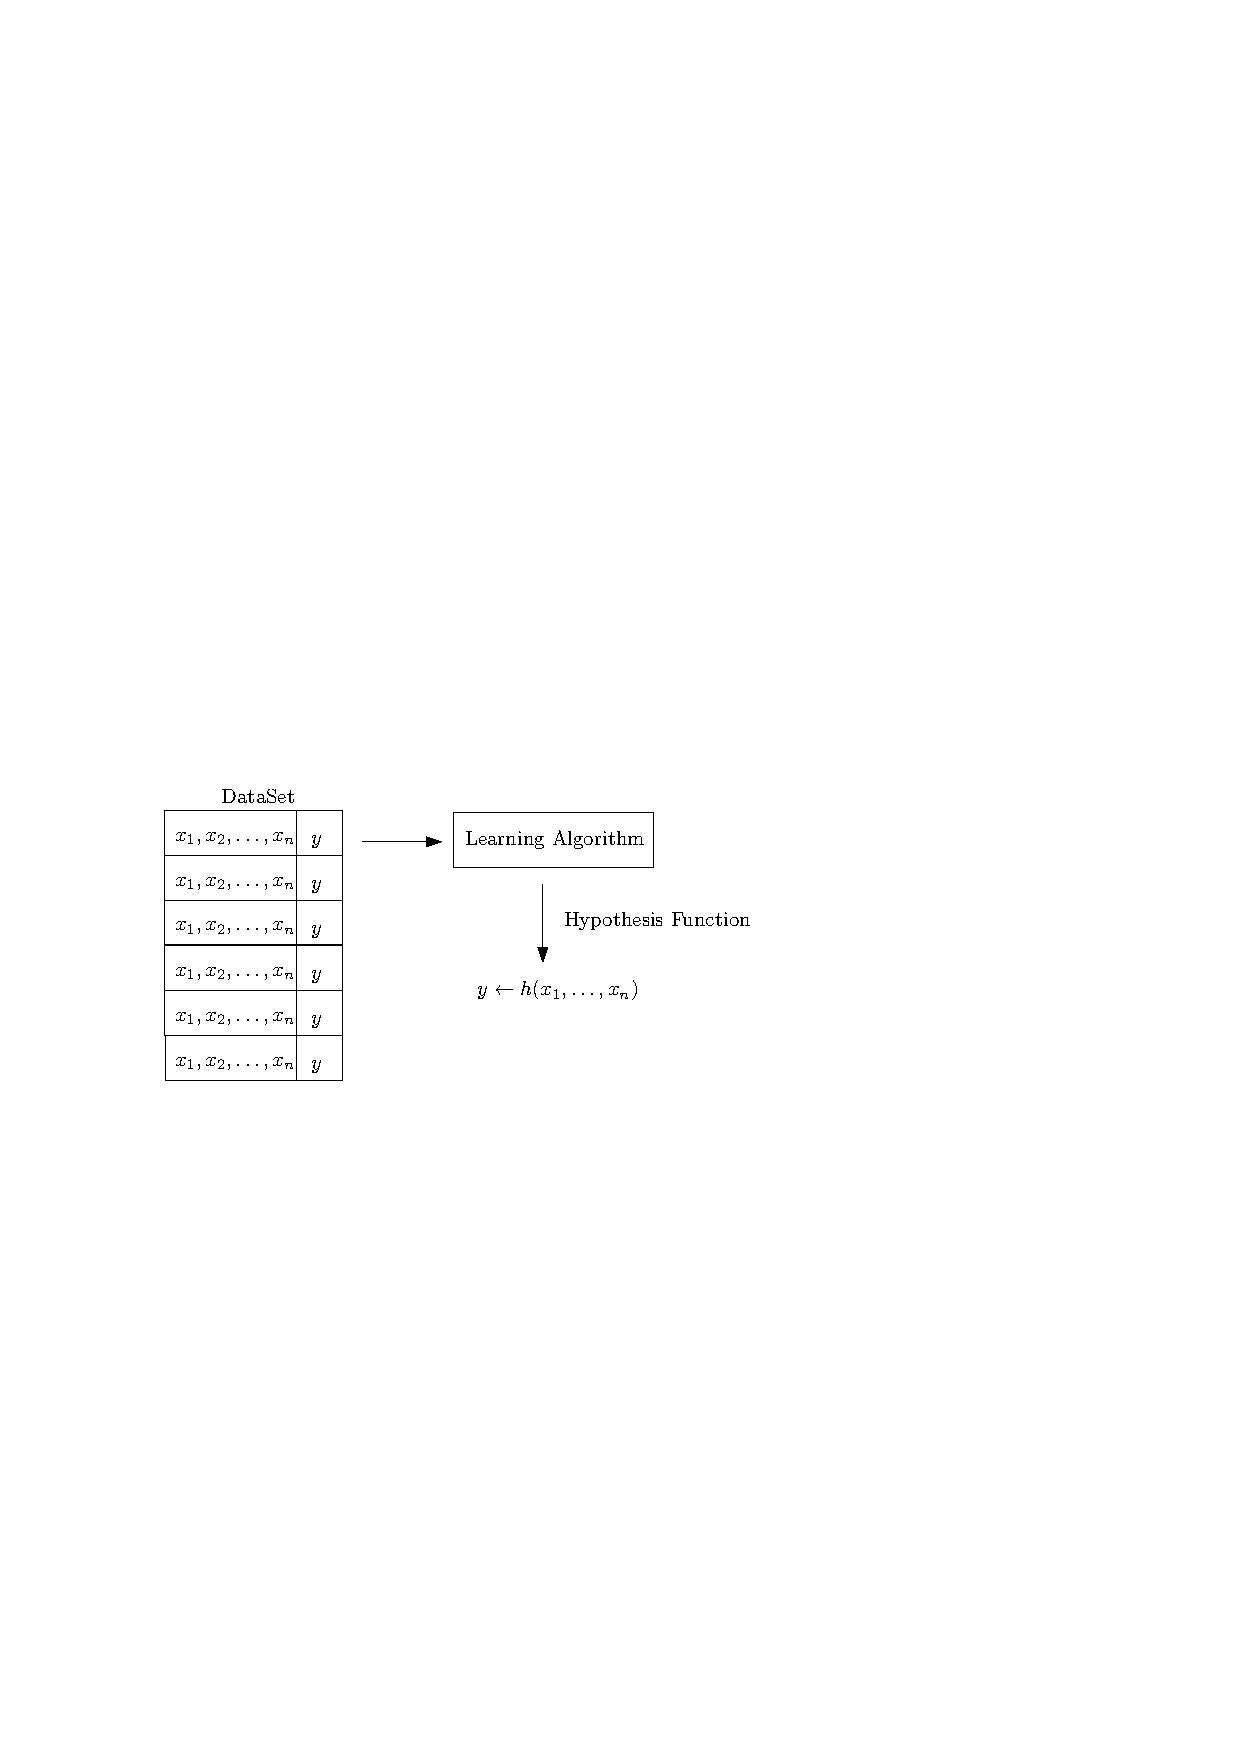
\includegraphics[scale=0.65]{pics/learning.pdf}
\end{figure}

} 
 
\end{frame}


\begin{frame}{Regresión Lineal Simple}
\scriptsize{
\begin{itemize}
 \item En la regresión lineal simple se tiene una única variable independiente $x$ para modelar la variable dependiente $\mathbf{y}$.

 \item Se asume la siguiente relación lineal entre la variables:

\begin{displaymath}
 y_i=\beta_{0}+\beta_{1}x_i +\epsilon_i \quad \forall i
\end{displaymath}

\item El parámetro $\beta_{0}$ representa el intercepto de la recta (el valor de $y$ cuando $x$ vale cero). 

\item El parámetro $\beta_{1}$ es la pendiente y representa el cambio de $\mathbf{y}$ cuando variamos el valor de $\mathbf{x}$. Entre mayor sea la magnitud de este parámetro mayor será la relación lineal entre las variables.

\item Los valores $\epsilon_{i}$ corresponden a los errores asociados al modelo.

\item Tenemos que encontrar una función lineal o recta $h_\beta$ que nos permita encontrar una estimación de $y$, $\hat{y}$ para cualquier valor de $x$ con el mínimo error esperado.

\begin{displaymath}
h(x)=\beta_{0}+\beta_{1}x 
\end{displaymath}


\end{itemize}


} 
 
\end{frame}



\begin{frame}{Mínimos de Cuadrados}
\scriptsize{
\begin{itemize}

 \item El método de mínimos cuadrados ordinarios  se usa para estimar $\hat{\beta}_{0}$ y $\hat{\beta}_{1}$ minimizando la suma de los errores cuadráticos (SSE) de los datos observados.

 \item Supongamos que tenemos $m$ observaciones de $\mathbf{y}$ y de $\mathbf{x}$,  calculamos la suma de los errores cuadráticos (SSE) o $E$ de error de la siguiente forma:

\begin{equation}
E = \sum_{i=1}^{m} (y_i-h(x_i))^2 =  \sum_{i=1}^{m} (y_i-\beta_{0}-\beta_{1}x_i)^2
\end{equation}

 \item Para encontrar los parámetros que minimizan el error calculamos las derivadas parciales de SSE respecto a $\beta_{0}$ y $\beta_{1}$. Luego igualamos las derivadas a cero y resolvemos la ecuación para despejar los parámetros.
 
 \begin{equation}
 \frac{\partial E}{ \partial \beta_0} = -2\sum_{i=1}^{m}(y_i-\beta_{0}-\beta_{1}x_i)=0
 \end{equation}

  \begin{equation}
 \frac{\partial E}{ \partial \beta_1} = -2\sum_{i=1}^{m}(y_i-\beta_{0}-\beta_{1}x)x_i=0
 \end{equation}



\end{itemize}



} 
\end{frame}

\begin{frame}{Mínimos Cuadrados (2)}
\scriptsize{
\begin{itemize}
 \item Del sistema de ecuaciones anterior se obtienen las soluciones normales:
  \begin{equation}
 \hat{\beta}_{1} = \frac{\sum_{i}^{m} (x_i-\overline{x})(y_i-\overline{y}) }{ \sum_{i}^{m} (x_i-\overline{x})^2}    
 \end{equation}

 \begin{equation}
 \hat{\beta}_{0} = \overline{y} -\beta_{1}\overline{x}    
 \end{equation}



\item El modelo ajustado representa la recta de mínimo error cuadrático.

\begin{figure}[h!]
	\centering
	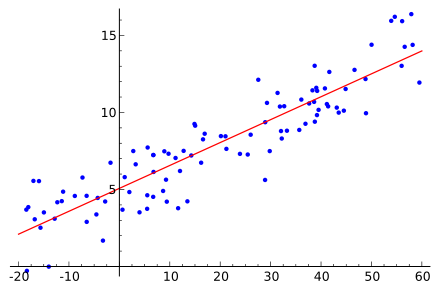
\includegraphics[scale=0.35]{pics/Linear_regression.png}
\end{figure}

\end{itemize}

} 
 
\end{frame}


\begin{frame}{Coeficiente de Determinación $R^2$}
\scriptsize{
\begin{itemize}
 \item Una vez ajustado nuestro modelo lineal debemos evaluar la calidad del modelo.
 \item Una medida muy común es el coeficiente de determinación $R^2$. 
 \item Para calcularlo debo calcular otros errores distintos a los errores cuadráticos SSE.
 \item Se define a la suma cuadrática total (SST) como el error predictivo cuando usamos la media $\overline{y}$ para predecir la variable de respuesta $y$ (es muy similar a la varianza de la variable):
 \begin{displaymath}
  \text{SST} = \sum_{i}^{m}(y_i-\overline{y})^2  
 \end{displaymath}
 \item Luego tenemos a la suma de los cuadrados explicada por el modelo (SSM) que nos indica la variabilidad de los valores predichos por el modelo respecto a la media:
 \begin{displaymath}
  \text{SSM} = \sum_{i}^{m}(\hat{y}_i-\overline{y})^2 
 \end{displaymath}
  
\end{itemize}

}
\end{frame}

\begin{frame}{Coeficiente de Determinación $R^2$ (2)}
\scriptsize{
\begin{itemize}
 \item Se define el coeficiente de determinación para un modelo lineal $R^2$ como:
 \begin{equation}
  R^2= \frac{\text{SSM}}{\text{SST}} = \frac{\sum_{i}^{m}(\hat{y}_i-\overline{y})^2 }{\sum_{i}^{m}(y_i-\overline{y})^2  }
 \end{equation}

 \item El coeficiente adquiere valores entre $0$ a $1$ y mientras más cercano a 1 sea su valor mayor sera la calidad del modelo.
 
 \item El valor de $R^2$ es equivalente a la correlación lineal (Pearsons) entre $y$ e $\hat{y}$ al cuadrado.
\begin{displaymath}
 R^2=\text{cor}(y,\hat{y})^2
\end{displaymath}
  
\end{itemize}


}
\end{frame}

\begin{frame}{Regresión Lineal Múltiple}
\scriptsize{
\begin{itemize}
 \item Supongamos que tenemos $n$ variables independientes: $x_1,x_2,\dots,x_n$.
 \item Intuitivamente, estas variables en conjunto podrían explicar de mejor manera la variabilidad de la variable de respuesta $\mathbf{y}$ que un modelo simple.
 \item Se define un modelo lineal multi-variado de la siguiente manera:
 \begin{displaymath}
 y_i=\beta_{0}+\beta_{1}x_{i,1}+ +\beta_{2}x_{i,2} + \cdots + \beta_{n}x_{i,n} +  \epsilon_i \quad \forall i \in \{1,m\}
\end{displaymath}
\item En el modelo multi-variado se extienden todas las propiedades del modelo lineal simple.

\item Se puede representar el problema de manera matricial:
\begin{displaymath}
 Y=X\beta+\epsilon
\end{displaymath}

\item Donde $Y$ es un vector de $m\times 1$ de variables de respuesta:

\begin{displaymath}
 Y =
 \begin{pmatrix}
  y_{1} \\
  y_{2}  \\
  \vdots  \\
  y_{m}
 \end{pmatrix}
\end{displaymath}






\end{itemize}
 

}
\end{frame}

\begin{frame}{Regresión Lineal Múltiple (2)}
\scriptsize{
\begin{itemize} 
\item $X$ es una matriz de $m \times (n+1)$ con las variables explicativas. Tenemos $m$ observaciones de las $n$ variables. La primera columna es constante igual a $1$ ($x_{i,0}=1 \quad \forall i$) para modelar la variable de intercepto $\beta_0$.

\begin{displaymath}
 X =
 \begin{pmatrix}
x_{1,0} &  x_{1,1} & x_{1,2} & \cdots & x_{1,n} \\
x_{2,0} &  x_{2,1} & x_{2,2} & \cdots & x_{2,n} \\
\vdots  &  \vdots  & \vdots  & \ddots & \vdots  \\
x_{m,0} &  x_{m,1} & x_{m,2} & \cdots & x_{m,n}
 \end{pmatrix}
\end{displaymath}

 \item Luego, $\beta$ es un vector de parámetros de $(n+1) \times 1$

\begin{displaymath}
 \beta =
 \begin{pmatrix}
  \beta_{0}  \\
  \beta_{1}  \\
  \vdots    \\
  \beta_{n} 
 \end{pmatrix}
\end{displaymath}





\end{itemize}
 

}
\end{frame}

\begin{frame}{Regresión Lineal Múltiple (2)}
\scriptsize{
\begin{itemize}
\item Finalmente, $\epsilon$ es un vector con los errores del modelo de $m \times 1$. 

\begin{displaymath}
 \epsilon =
 \begin{pmatrix}
  \epsilon_{1}  \\
  \epsilon_{2}  \\
  \vdots    \\
  \epsilon_{m} 
 \end{pmatrix}
\end{displaymath}

\item Usando la notación matricial, podemos ver que la suma de los errores cuadráticos (SSE) se puede expresar como:
\begin{displaymath}
 \text{SSE} = (Y - X\beta)^{T}(Y-X\beta)
\end{displaymath}

\item Minimizando esta expresión derivando el error en función de $\beta$ e igualando a cero se llega a las ecuaciones normales:

\begin{displaymath}
   \hat{\beta} = (X^{T}X)^{-1} X^{T}Y
\end{displaymath}


\end{itemize}


}

\end{frame}

\begin{frame}{Supuestos del Modelo Lineal}
\scriptsize{





Cada vez que ajustamos un modelo lineal estamos asumiendo implícitamente ciertos supuestos sobre los datos. 


\begin{block}{Supuestos}
\begin{enumerate}
\item Linealidad: la variable de respuesta se relaciona linealmente con los atributos. 
\item Normalidad: los errores tienen distribución normal de media cero: $\epsilon_{i} \sim N(0,\sigma^2)$ 
\item Homocedasticidad: los errores tienen  varianza constante (mismo valor $\sigma^2$).
\item Independencia: los errores son independientes entre sí.
 
\end{enumerate}
 
\end{block}

} 
\end{frame}


\begin{frame}{Interpretación Probabilística}
\scriptsize{
\begin{itemize}
 \item Considerando los supuestos anteriores podemos ver que la densidad de probabilidad (PDF) de los errores $\epsilon$ esta definida por una normal de media cero y varianza constante:
 \begin{displaymath}
  \text{PDF}(\epsilon_{i})=\frac{1}{\sqrt{2\pi} \sigma} \exp \left(- \frac{\epsilon_{i}^{2}}{2\sigma^2}\right)
 \end{displaymath}
 \item Esto implica que:
  \begin{displaymath}
  \text{PDF}(y_i|x_{i};\beta)=\frac{1}{\sqrt{2\pi} \sigma} \exp \left(- \frac{(y_i - h_{\beta}(x_{i}) )^{2}}{2\sigma^2}\right)
 \end{displaymath}
 \item Lo que implica que la distribución de $\mathbf{y}$ dada los valores de $\mathbf{x}$ y parametrizada por $\beta$ sigue una distribución normal.
 \item Luego si uno estima los parámetros de $\beta$ usando una técnica de estimación llamada máxima verosimilitud llega a los mismos resultados que haciendo estimación por mínimos cuadrados.
 \item Esto nos dice que cuando estimamos los parámetros del modelo usando mínimos cuadrados estamos realizando las mismas hipótesis probabilísticas mencionados anteriormente.
 

\end{itemize}


}
 
\end{frame}

\begin{frame}[fragile]{Regresiones en R}
\scriptsize{
\begin{itemize}
 \item En R lo modelos lineales se crean con el comando \verb+lm+ que recibe como parámetro una fórmula de la forma \verb+y~x+ ($y=f(x)$).
 \item Vamos a trabajar con el dataset \verb+USArrests+ que tiene información sobre los arrestos ocurridos en Estados Unidos el año 1973. 
 \item Cada observación corresponde a un estado.
 \item Tiene las siguientes variables:
 \begin{enumerate}
 \scriptsize{
  \item \textbf{Murder}:  arrestos por homicidio (por 100.000 habitantes).
  \item \textbf{Assault} : arrestos por asalto (por 100.000 habitantes).
  \item \textbf{UrbanPop}: porcentaje de la población total del estado.
  \item \textbf{Rape}: arrestos por violación (por 100.000 habitantes).
  }
 \end{enumerate}
 
\item Para ver si vale la pena hacer un análisis de regresión lineal vemos las correlaciones lineales entre las variables: 

 \begin{verbatim}
> data(USArrests)
> attach(USArrests)
> cor(USArrests)
             Murder   Assault   UrbanPop      Rape
Murder   1.00000000 0.8018733 0.06957262 0.5635788
Assault  0.80187331 1.0000000 0.25887170 0.6652412
UrbanPop 0.06957262 0.2588717 1.00000000 0.4113412
Rape     0.56357883 0.6652412 0.41134124 1.0000000  
 \end{verbatim}

 
 
 
\end{itemize}
 
 
 
 
} 
\end{frame}

\begin{frame}[fragile]{Regresiones en R (2)}
\scriptsize{
\begin{itemize}
 \item Podemos ver que hay una correlación positiva importante entre \verb+Murder+ y \verb+Assault+.
 \item Vamos a modelar los asesinatos en función de los asaltos usando una regresión lineal simple:
 \begin{displaymath}
  \text{Murder}(\text{Assault})=\beta_0+\beta_1*\text{Assault}
 \end{displaymath}
 \begin{verbatim}
> reg1<-lm(Murder~Assault,USArrests)
> reg1

Call:
lm(formula = Murder ~ Assault, data = USArrests)

Coefficients:
(Intercept)      Assault  
    0.63168      0.04191    
 \end{verbatim}
 
 \item Podemos ver que los coeficientes del modelo son $\beta_{0}=0.632$ y $\beta_{1}=0.042$. 
 
 


\end{itemize}
 
 
 
} 
\end{frame}

\begin{frame}[fragile]{Regresiones en R (3)}
\scriptsize{
\begin{itemize}
 \item Podemos acceder directamente a los coeficientes y guardarlos en una variable:
 \begin{verbatim}
> reg1.coef<-reg1$coefficients
> reg1.coef
(Intercept)     Assault 
 0.63168266  0.04190863 
 \end{verbatim}
 
\item Podemos ver diversos indicadores sobre el modelo lineal con el comando \textbf{summary}:
 
\begin{verbatim}
> summary(reg1)
Residuals:
    Min      1Q  Median      3Q     Max 
-4.8528 -1.7456 -0.3979  1.3044  7.9256 

Coefficients:
            Estimate Std. Error t value Pr(>|t|)    
(Intercept) 0.631683   0.854776   0.739    0.464    
Assault     0.041909   0.004507   9.298  2.6e-12 ***
---
Signif. codes:  0 ‘***’ 0.001 ‘**’ 0.01 ‘*’ 0.05 ‘.’ 0.1 ‘ ’ 1

Residual standard error: 2.629 on 48 degrees of freedom
Multiple R-squared:  0.643,	Adjusted R-squared:  0.6356 
F-statistic: 86.45 on 1 and 48 DF,  p-value: 2.596e-12

\end{verbatim}
 
 \end{itemize}
 
 


} 
\end{frame}


\begin{frame}[fragile]{Regresiones en R (4)}
\scriptsize{
\begin{itemize}
 \item Vemos que el coeficiente de determinación $R^2$ tiene un valor de $0.643$ lo cual no es tan bueno pero aceptable.
 
 
  \item Podemos concluir que el nivel de asaltos si bien provee información útil para modelar una parte de la variabilidad del nivel de homicidios no es suficiente para construir un modelo altamente confiable. 
  
  \item Puedo guardar los resultados del comando \verb+summary+ en una variable y así acceder directamente al coeficiente de determinación:
\begin{verbatim}
> sum.reg1<-summary(reg1)
> sum.reg1$r.squared
[1] 0.6430008   
\end{verbatim}

\item También puedo acceder a los valores ajustados que son los valores predichos por mi modelo para los datos usados:
\begin{verbatim}
> reg1$fitted.values
       Alabama         Alaska        Arizona       Arkansas        
     10.522119      11.653652      12.952819       8.594322      
\end{verbatim}
 
 \end{itemize}
 

} 
\end{frame}



\begin{frame}[fragile]{Regresiones en R (5)}
\scriptsize{
\begin{itemize}
 \item Podemos ver que la correlación lineal al cuadrado entre mis valores ajustados y los observados para la variable de respuesta es equivalente al coeficiente de determinación:
 
 \begin{verbatim}
> cor(Murder,reg1$fitted.values)^2
[1] 0.6430008
 \end{verbatim}

\item Supongamos ahora que conozco el nivel de asalto de dos estados en otro período para dos lugares pero no conozco el nivel de homicidios.

\item Podría usar mi modelo lineal para predecir el nivel de de homicidios.

\item Para hacerlo en R debo usar el comando \verb+predict.lm+ que recibe el modelo lineal y un data.frame con los datos nuevos:
\begin{verbatim}
> nuevos.arrestos<-data.frame(Assault=c(500,12))
> predict.lm(object=reg1,newdata=nuevos.arrestos)
        1         2 
21.585997  1.134586 
> # Esto es equivalente a:
> reg1.coef[1]+reg1.coef[2]*nuevos.arrestos
    Assault
1 21.585997
2  1.134586 
\end{verbatim}

 
 \end{itemize}
 

} 
\end{frame}


\begin{frame}[fragile]{Regresiones en R (6)}
\scriptsize{
\begin{itemize}
 \item Ahora estudiaremos una regresión lineal múltiple.
 \item Podemos ver que la variable \textbf{Rape} que representa el nivel de violaciones tiene una correlación menor con el número de asaltos y con el número de homicidios que la correlación que presentan estas dos variables entre sí.
 \item Vamos a ajustar el siguiente modelo lineal multi-variado:
 \begin{displaymath}
 \text{Rape}=\beta_{0}+\beta_{1}*\text{Assault}+\beta_{2}*\text{Murder}
 \end{displaymath}
 \item En R para agregar más variables al modelo lineal las agregamos con el signo \textbf{+} :
\begin{verbatim}
reg2<-lm(Rape~Assault+Murder,USArrests)
\end{verbatim}



 
 \end{itemize}
 

} 
\end{frame}


\begin{frame}[fragile]{Regresiones en R (7)}
\scriptsize{

\begin{verbatim}
> summary(reg2)

Residuals:
    Min      1Q  Median      3Q     Max 
-17.243  -3.171  -1.171   3.281  18.511 

Coefficients:
            Estimate Std. Error t value Pr(>|t|)    
(Intercept)  8.35011    2.32912   3.585 0.000799 ***
Assault      0.06716    0.02044   3.286 0.001927 ** 
Murder       0.18155    0.39108   0.464 0.644619    
---
Signif. codes:  0 ‘***’ 0.001 ‘**’ 0.01 ‘*’ 0.05 ‘.’ 0.1 ‘ ’ 1

Residual standard error: 7.124 on 47 degrees of freedom
Multiple R-squared:  0.4451,	Adjusted R-squared:  0.4215 
F-statistic: 18.85 on 2 and 47 DF,  p-value: 9.755e-07

\end{verbatim}

\begin{itemize}
\item En este caso el coeficiente de determinación es bajo. Por lo que tendremos baja confianza en la calidad del modelo.
 \end{itemize}
 

} 
\end{frame}

\begin{frame}[fragile]{Regresiones en R (8)}
\scriptsize{
\begin{itemize}
 \item Cuando teníamos una regresión simple podíamos ver el modelo ajustado como una recta.
 \item Ahora que tenemos dos variables independientes podemos ver el modelo ajustado como un plano.
 \item Si tuviésemos más variables independientes nuestro modelo sería un hiper-plano.
 \item Podemos graficar en R el plano de nuestro modelo lineal de dos variables independientes y una dependiente de la siguiente manera:
 \end{itemize}

\begin{verbatim}
library("scatterplot3d")
s3d <- scatterplot3d(USArrests[,c("Assault","Murder","Rape")],
                     type="h", highlight.3d=TRUE,
                     angle=55, scale.y=0.7, pch=16, 
                     main="Rape~Murder+Rape")
s3d$plane3d(reg2, lty.box = "solid")

\end{verbatim}




} 
\end{frame}

\begin{frame}{Regresiones Lineales en R (9)}
 
\begin{figure}[h!]
	\centering
	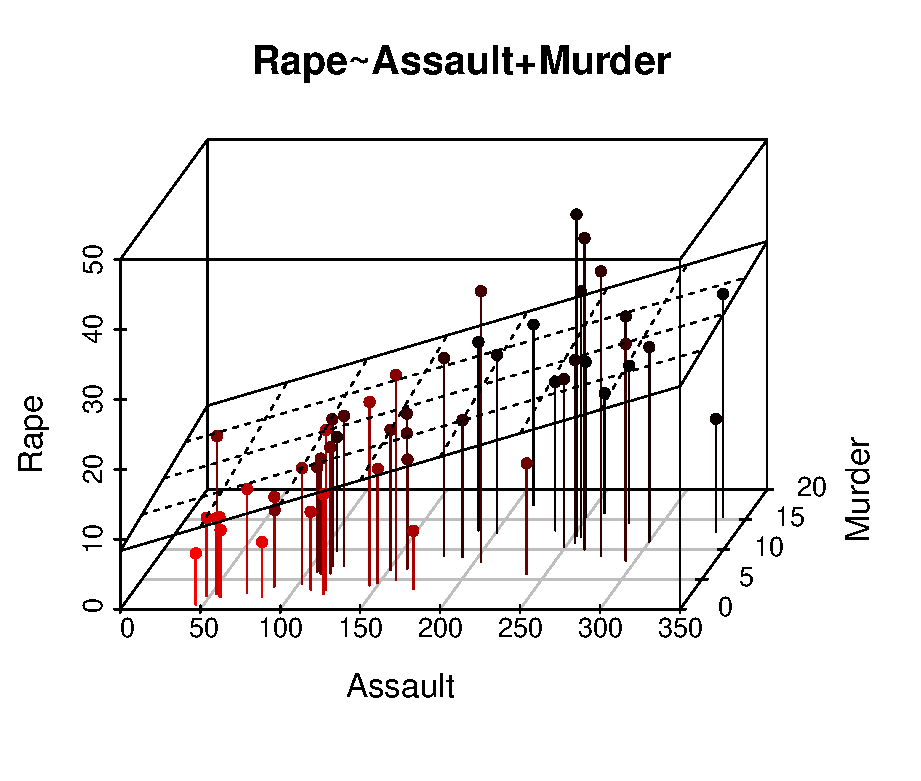
\includegraphics[scale=0.6]{pics/reg3d.pdf}
\end{figure}
 
\end{frame}



\begin{frame}{FOUR CARDINAL RULES OF STATISTICS by Daniela Witten}
\scriptsize{
\begin{itemize}
% source: https://twitter.com/daniela_witten/status/1312180955801505794
 \item ONE:  CORRELATION DOES NOT IMPLY CAUSATION.  Yes, I know you know this, but it’s so easy to forget! Yeah, YOU OVER THERE, you with the p-value of 0.0000001 — yes, YOU!! That’s not causation.
 \item No matter how small the p-value for a regression of IQ onto shoe size is, that doesn’t mean that big feet cause smarts!!  It just means that grown-ups tend to have bigger feet and higher IQs than kids.
 \item So, unless you can design your study to uncover causation (very hard to do in most practical settings — the field of causal inference is devoted to understanding the settings in which it is possible), the best you can do is to discover correlations.  Sad but true.
 \item TWO:  A P-VALUE IS JUST A TEST OF SAMPLE SIZE.  Read that again — I mean what I said!  If your null hypothesis doesn't hold (and null hypotheses never hold IRL) then the larger your sample size, the smaller your p-value will tend to be.
 \item If you’re testing whether mean=0 and actually the truth is that mean=0.000000001, and if you have a large enough sample size, then YOU WILL GET A TINY P-VALUE.
 \item Why does this matter? In many contemporary settings (think: the internet), sample sizes are so huge that we can get TINY p-values even when the deviation from the null hypothesis is negligible. In other words, we can have STATISTICAL significance w/o PRACTICAL significance.
 \end{itemize}

} 
\end{frame}

\begin{frame}{FOUR CARDINAL RULES OF STATISTICS by Daniela Witten}
\scriptsize{
\begin{itemize}
 \item Often, people focus on that tiny p-value, and the fact that the effect is of **literally no practical relevance** is totally lost.
 \item This also means that with a large enough sample size we can reject basically ANY null hypothesis (since the null hypothesis never exactly holds IRL, but it might be “close enough” that the violation of the null hypothesis is not important). 
 \item Want to write a paper saying Lucky Charms consumption is correlated w/blood type? W/a large enough sample size, you can get a small p-value.  (Provided there’s some super convoluted mechanism with some teeny effect size… which there probably is, b/c IRL null never holds)
\item THREE:  SEEK AND YOU SHALL FIND. If you look at your data for long enough, you will find something interesting, even if only by chance! 
In principle, we know that we need to perform a correction for multiple testing if we conduct a bunch of tests.
\item But in practice, what if we decide what test(s) to conduct AFTER we look at data?  Our p-value will be misleadingly small because we peeked at the data.  Pre-specifying our analysis plan in advance keeps us honest… but in reality, it’s hard to do!!!
\item Everyone is asking me about the mysterious and much-anticipated fourth rule of statistics. The answer is simple: we haven’t figured it out yet.... that’s the reason we need to do research in statistics
\end{itemize}

} 
\end{frame}



\begin{frame}[allowframebreaks]\scriptsize
\frametitle{Bilbiografía}
\begin{thebibliography}{8}

\bibitem{Assaad2008}
L. Wasserman \emph{All of Statistics: A Concise Course in Statistical Inference}, Springer Texts in Statistics, 2005.
\end{thebibliography}


\end{frame}




%%%%%%%%%%%%%%%%%%%%%%%%%%%

\end{document}
